 \documentclass{beamer}

%\usecolortheme[RGB={170,130,220}]{structure}
\setbeamertemplate{items}[ball]
\setbeamertemplate{blocks}[rounded][shadow=true]
%\beamertemplateshadingbackground{yellow!15}{magenta!15}
\usetheme{Singapore}

\usepackage{amsmath, amsthm, amssymb, enumerate, natbib}
\usepackage{graphicx, epsfig}
\usepackage{setspace}
\usepackage{color}
\usepackage{subfigure}

\definecolor{darkgreen}{rgb}{0,0.4,0}
\definecolor{cgreen}{rgb}{0,0.5,0}
\definecolor{darkblue}{rgb}{0,0,0.6}
\definecolor{darkred}{rgb}{0.7,0,0.1}
\definecolor{lessdarkgreen}{rgb}{0.2,0.5,0}
\definecolor{darkerred}{rgb}{0.5,0.1,0.05}
\definecolor{lessdarkred}{rgb}{0.8,0,0}
\definecolor{purple}{rgb}{0.8,.0,0.9}
\definecolor{darkpurple}{rgb}{0.45,.0,1.0}
\definecolor{darkerpurple}{rgb}{0.5,.2,.9}
\definecolor{brightred}{rgb}{1,0,0}


\mode<presentation> {
  \usetheme{Singapore}
  % or ...

  \setbeamercovered{transparent}
  % or whatever (possibly just delete it)
}

\usepackage[english]{babel}
\usepackage[latin1]{inputenc}
\usepackage{times}
\usepackage[T1]{fontenc}
\usepackage{framed}

\newtheorem{proposition}[theorem]{Proposition}
\theoremstyle{definition}
\newtheorem{remark}[theorem]{Remark}
\newtheorem{algorithm}[theorem]{Algorithm}

\begin{document}


\title{\LARGE{Analyzing Flow-Cytometry Count Data with Regression Mixtures}}

\author{\large{\textbf{Amit Meir}} \\ \emph{University of Washington} \\ \vspace{1 cm} Joint work with \\ \vspace{0.1 cm} \textbf{Raphael Gottardo} and \textbf{Greg Finak} 
\\ \emph{Hutchinson Cancer Research Center}}


\vspace{1 cm}

%%%%%%%%%%%%%%%%%%%%%%%%%%%%%%%%%%%%%%%%%

\begin{frame}[plain]
  \titlepage
\end{frame}


%%%%%%%%%%%%%%%%%%%%%%%%%%%%%%%%%%%%%%%%%%%%%%%

\begin{frame}
\frametitle{Outline}
\begin{enumerate}
\item \textbf{Introduction} to Flow-Cytometry
\vspace{0.3 cm}
\item \textbf{Motivation}
	\begin{itemize}
	\item Existing methods
	\item Why a regression model?
	\end{itemize}
\vspace{0.3 cm}
\item \textbf{Models}:
	\begin{itemize}
	\item A Marginal Model
	\item A Joint HMRF model
	\end{itemize}
	\vspace{0.3 cm}
\item \textbf{Data analysis}
	\begin{itemize}
	\item RV144 HIV Vaccine Trial
	\item Controlled Human Malaria Infection Study.
	\end{itemize}

\vspace{0.3 cm}
\item  \textbf{Computation} (time permitting)
\end{enumerate}
\end{frame}

%%%%%%%%%%%%%%%%%%%%%%%%%%%%%%%%%%%%%%%

\begin{frame}
\frametitle{The RV144 HIV Vaccine Trial}
\begin{center}
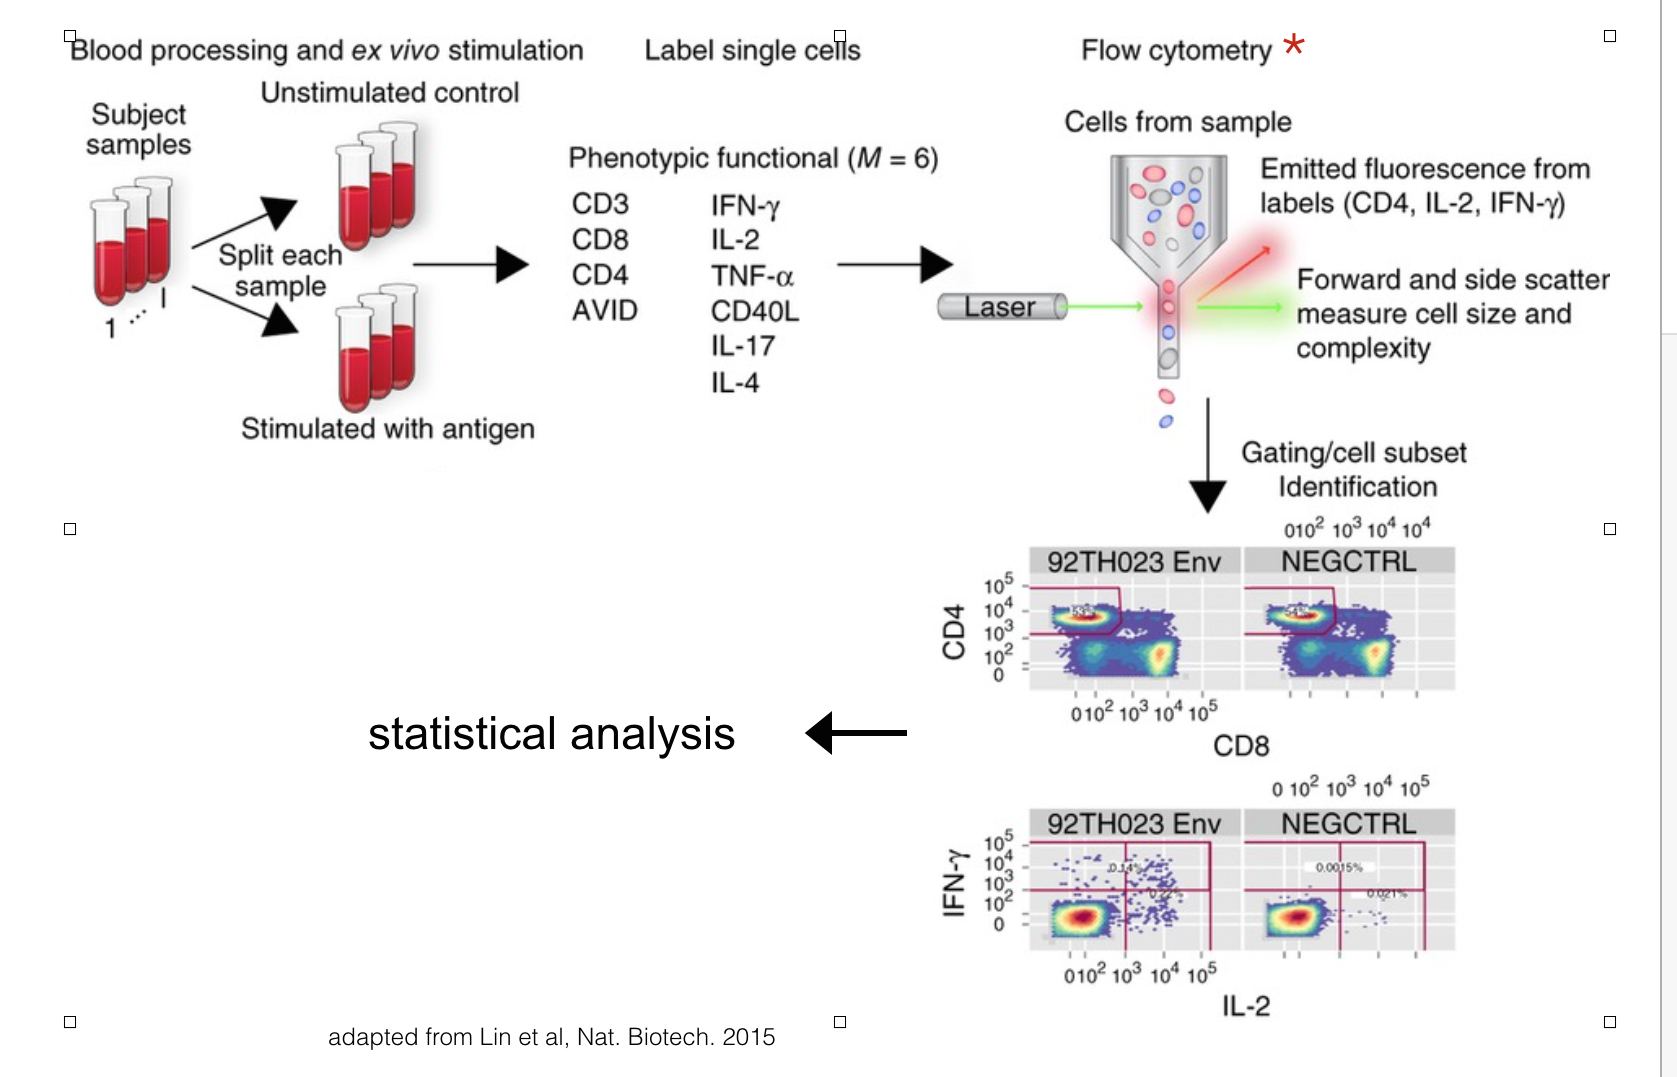
\includegraphics[scale=0.4]{figures/flowcytintro}
\end{center}
\end{frame}


%%%%%%%%%%%%%%%%%%%%%%%%%%%%%%%%%%%%%%%%%%%%%%%

\begin{frame}
\frametitle{The RV144 HIV Vaccine Trial}
\begin{figure}[]
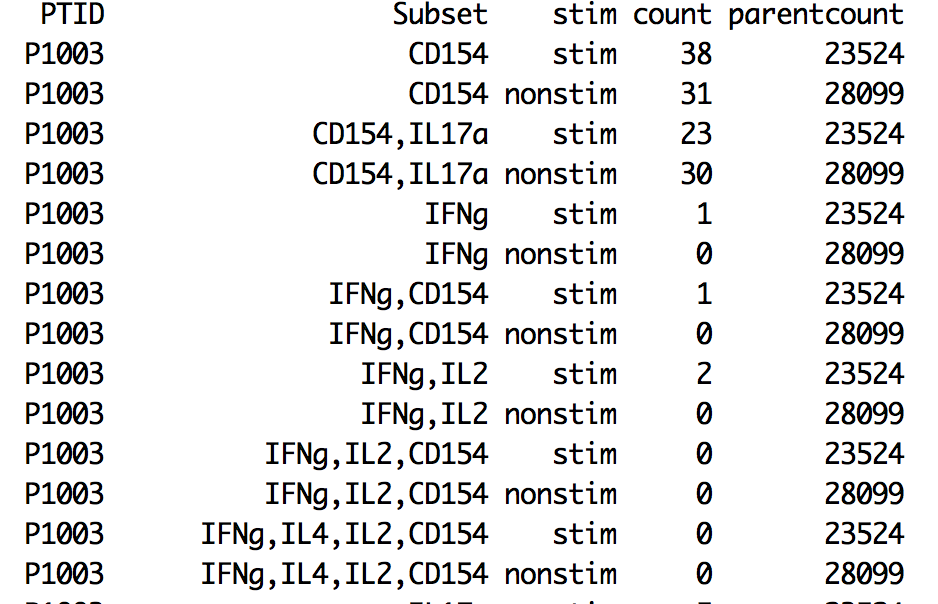
\includegraphics[width=12 cm]{figures/datasetExample} \caption{}
\end{figure}
\end{frame}

%%%%%%%%%%%%%%%%%%%%%%%%%%%%%%%%%%%%%%%%%%%%%%%

\begin{frame}
\frametitle{The RV144 HIV Vaccine Trial}
\begin{itemize}
\item \textbf{262 Subjects}
	\begin{itemize}
	\item 226 Cases
	\item 36 Controls
	\end{itemize}
\vspace{0.2 cm}
\item \textbf{2 Types of stimulus} 
	\begin{itemize}
	\item HIV antigen
	\item Negative control
	\end{itemize}
\vspace{0.2 cm}
\item \textbf{6 types of cytokines.} 
\end{itemize}
\end{frame}

%%%%%%%%%%%%%%%%%%%%%%%%%%%%%%%%%%%%%%%%

\begin{frame}
\frametitle{Marginal Counts for RV144}
\begin{center}
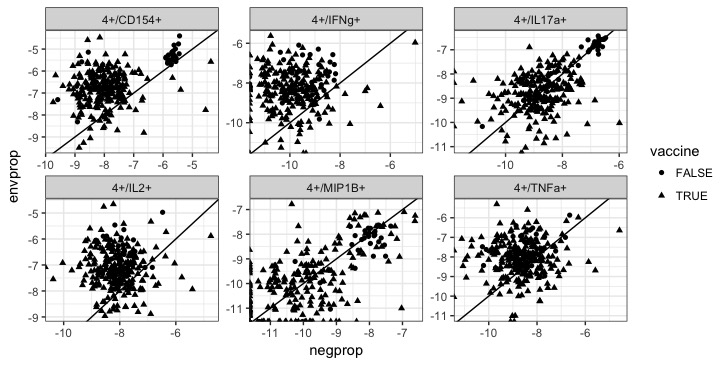
\includegraphics[scale=0.4]{figures/marginalScatterNoPost}
\end{center}
\end{frame}

%%%%%%%%%%%%%%%%%%%%%%%%%%%%%%%%%%%%%%%%

\begin{frame}
\frametitle{Motivation: COMPASS}
\begin{center}

\includegraphics[scale=0.18]{figures/compassCaption}
\end{center}

\pause
\textbf{Or in general, with immune response.}
\end{frame}

%%%%%%%%%%%%%%%%%%%%%%%%%%%%%%%%%%%%%%%%

\begin{frame}
\frametitle{How do current methods work? (Approximately)}
Current models are baseline/stimulation models. 
\begin{itemize}
\item  Unstimulated blood sample are compared stimulated ones.
\end{itemize}
\vspace{0.3 cm}

\pause
For the unstimulated sample of the $i$th subject out of $n$, we sample a count proportion:
$$
p_{i0} \sim \text{Dirichlet}(\alpha_{0},\beta_{0}),
$$$$
y_{i0} \sim \text{Multinomial}(N_{i0}, p_{i0}).
$$


\vspace{0.3 cm}
\pause
Let $k_i \in \{0,1\}^{p}$ indicate in which subsets $i$ responds:
$$
k_{ij} \sim \text{Ber}(w_j),
$$$$
p_{i1,\tau = 0} \sim \delta(p_{i0,\tau = 0}), \;\;\;\;
p_{i1, \tau = 1} | p_{i0,\tau = 0}  \propto \text{Dirichlet}(\alpha_1, \beta_{1})
$$$$
y_{i1} \sim \text{Multinomial}(N_{i1}, p_{i1})
$$
\end{frame}

%%%%%%%%%%%%%%%%%%%%%%%%%%%%%%%%%%%%%%%%%%%%%%%

\begin{frame}
\frametitle{Controlled Human Malaria Infection Study}
\begin{itemize}
\item 9 subjects were infected with Malaria.
	\begin{itemize}
	\item +3 controls.
	\end{itemize}
	\vspace{0.75 cm}
	
\item Blood samples were collected at 6 time points.
	\begin{itemize}
	\item Day 0, day 9, blood  parasitemia, Day 28, Day 56, Day 168.
	\end{itemize}
	\vspace{0.75 cm}

\item Two types of stimulation:
	\begin{itemize}
	\item Infected/uninfected blood-cells.
	\end{itemize}
	\vspace{0.75 cm}
	
\item 53 cell subsets.
	\begin{itemize}
	\item (10 types of cytokines in 8 cell-types)
	\end{itemize} 
\end{itemize}
\end{frame}

%%%%%%%%%%%%%%%%%%%%%%%%%%%%%%%%%%%%%%%%

\begin{frame}
\frametitle{Controlled Human Malaria Infection Study}
\begin{center}
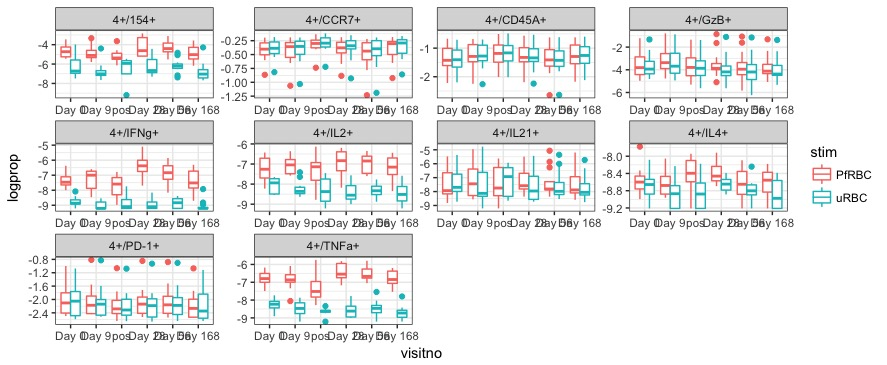
\includegraphics[scale=0.38]{figures/malariaBoxplotsFourPlus}
\end{center}
\end{frame}

%%%%%%%%%%%%%%%%%%%%%%%%%%%%%%%%%%%%%%%%

\begin{frame}
\frametitle{Motivation - A Regression Model}
\begin{itemize}
\item We want to be able to include covariates:
	\begin{itemize}
	\item Batch effects.
	\item Other covariates such as age, gender...
	\end{itemize}

\pause
\vspace{0.7 cm}
\item Longitudal data.

\vspace{0.7 cm}
\item More than one stimulation.

\pause
\vspace{0.7 cm}
\item Explicit dependence model:
	\begin{itemize}
	\item For the observed proportions.
	\item For response/non-response.
	\end{itemize}
\end{itemize}
\end{frame}

%%%%%%%%%%%%%%%%%%%%%%%%%%%%%%%%%%%%%%%%%%%%%%%

\begin{frame}
\frametitle{Motivation - Unique Challanges}
\begin{itemize}
\item \textbf{Dependence}
	\begin{itemize}
	\item Within sample between cell subsets.
	\item Within subject / across time.  
	\end{itemize}
\vspace{0.76 cm}
\item \textbf{Heterogenous treatment effect}
\vspace{0.76 cm}
\item \textbf{Over-dispersed Binomial counts}
\end{itemize}
\end{frame}

%%%%%%%%%%%%%%%%%%%%%%%%%%%%%%%%%%%%%%%%%%%%%%%

\begin{frame}
\frametitle{A Marginal Model - Single Subset}
\begin{framed}
Indexing: \textbf{i}-subject, \textbf{t}- stimulation/time-point.
\end{framed}

Overdispersion $\Rightarrow$ Beta Binomial Model.
$$
\text{logit}(\mu_{it}) = X_{it} \beta,
$$$$
p_{it} \sim \text{Beta}(M\mu, M(1 - \mu)),
$$$$
y_{it} \sim \text{Binom}(N_{it}, p_{it})
$$
\end{frame}

%%%%%%%%%%%%%%%%%%%%%%%%%%%%%%%%%%%%%%%%%%%%%%%

\begin{frame}
\frametitle{A Marginal Model - Single Subset}
\begin{framed}
Indexing: \textbf{i}-subject, \textbf{t}- stimulation/time-point.
\end{framed}
Dependence $\Rightarrow$ `random' subject baseline:
$$
\nu_i \sim N(0, \sigma^{2})
$$$$
\text{logit}(\mu_{it}) = X_{it} \beta + \nu_i
$$$$
p_{it} \sim \text{Beta}(M\mu, M(1 - \mu)),
$$$$
y_{it} \sim \text{Binom}(N_{it}, p_{it})
$$

\end{frame}

%%%%%%%%%%%%%%%%%%%%%%%%%%%%%%%%%%%%%%%%%%%%%%%]

\begin{frame}
\frametitle{A Marginal Model - Single Subset}
\begin{framed}
Indexing: \textbf{i}-subject, \textbf{t}- stimulation, \textbf{k}- cluster.
\end{framed}

Non-response $\Rightarrow$ Mixture-Model:
$$
k \sim Ber(\theta),
$$$$
\text{logit}(\mu_{itk}) = X_{it} \beta + T_{it}\tau_{k} + \nu_i,
$$
	\begin{itemize}
	\item $T$ a matrix of covariates related to the treatment.
	\item $\tau_k$ equals $0$ if $k=0$ or $\tau\neq0$ if $k = 1$.
	\end{itemize}
\end{frame}

%%%%%%%%%%%%%%%%%%%%%%%%%%%%%%%%%%%%%%%%%%%%%%%]

\begin{frame}
\frametitle{A Marginal Model - Recap}
\begin{framed}
Indexing: \textbf{i}-subject, \textbf{t}- stimulation, \textbf{k}- cluster.
\end{framed}
$$
\nu_i \sim N(0, \sigma^{2}),
$$$$
k \sim Ber(\theta),
$$$$
\text{logit}(\mu_{itk}) = X_{it} \beta + T_{it}\tau_{k} + \nu_i,
$$$$
p_{it} \sim \text{Beta}(M\mu, M(1 - \mu)),
$$$$
y_{it} \sim \text{Binom}(N_{it}, p_{it})
$$

\vspace{0.3 cm}
\textbf{Model can be estimated via an EM algorithm}
\end{frame}

%%%%%%%%%%%%%%%%%%%%%%%%%%%%%%%%%%%%%%%%%%%%%%%]

\begin{frame}
\frametitle{Wellness of Fit Evaluation}
How do we evaluate the model?
\begin{itemize}
\item We fit the model without information regarding the true treatment allocation. 
\vspace{0.3 cm}
\item The model should be able to discriminate between vaccinees and placebos.
\vspace{0.3 cm}
\pause
\item We use three type of figures:
	\begin{itemize}
	\item Scatter plots w/classification information.
	\item Receiver-Operator Curves.
	\item False Detection Rates. 
	\end{itemize}
\end{itemize}
\end{frame}

%%%%%%%%%%%%%%%%%%%%%%%%%%%%%%%%%%%%%%%%%%%%%%%]

\begin{frame}
\frametitle{Marginal Model - Results}
\begin{center}
\begin{figure}[]
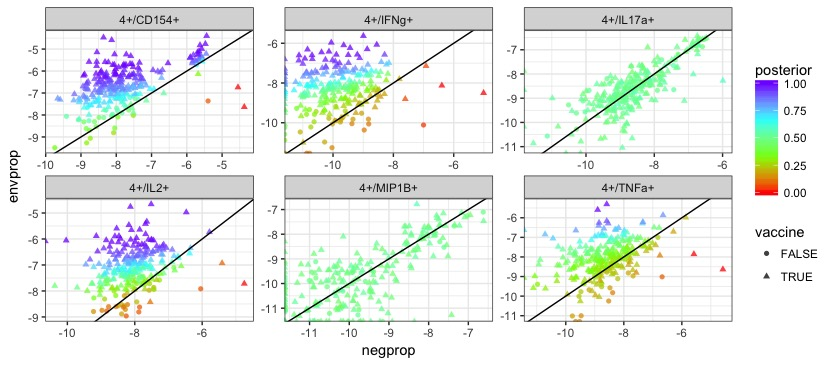
\includegraphics[width=12 cm]{figures/marginalBooleansIndependenceScatter}
 \caption{Posterior Probabilities for RV144 dataset - Independence Model}
\end{figure}
\end{center}
\end{frame}

%%%%%%%%%%%%%%%%%%%%%%%%%%%%%%%%%%%%%%%%%%%%%%%]

\begin{frame}
\frametitle{Comparison w/ MIMOSA - Finak et al. (2013) }
\begin{figure}[]
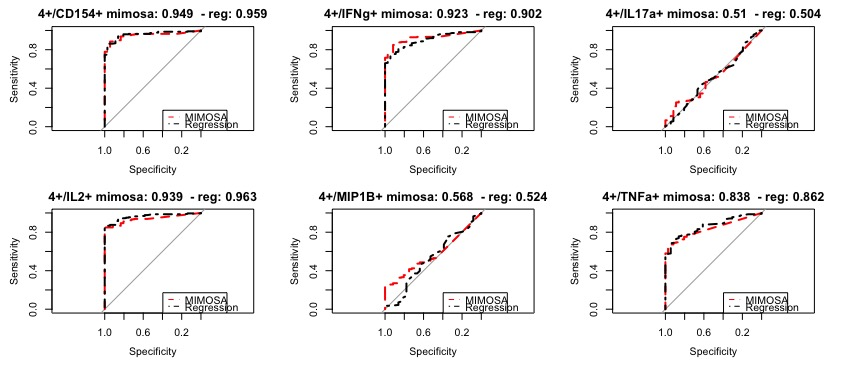
\includegraphics[width=11 cm]{figures/mimosaComparisonROC} 
\caption{Comparison with MIMOSA (univariate COMPASS)}
\end{figure}
\end{frame}

%%%%%%%%%%%%%%%%%%%%%%%%%%%%%%%%%%%%%%%%%%%%%%%]

\begin{frame}
\frametitle{Comparison w/ MIMOSA - Finak et al. (2013) }
\begin{figure}[]
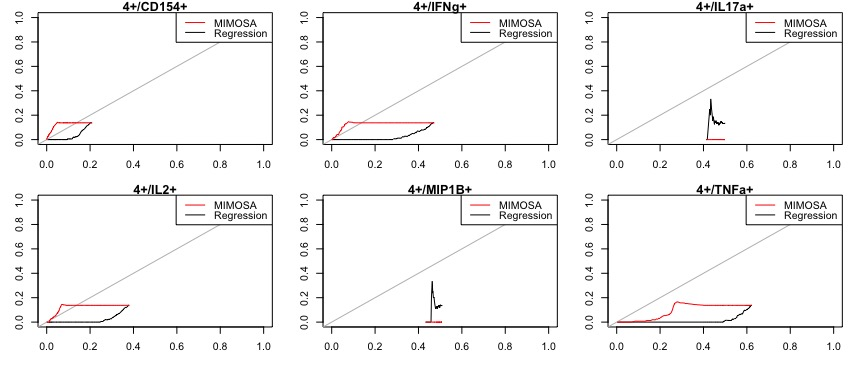
\includegraphics[width=11 cm]{figures/mimosaComparisonFDR} 
\caption{Comparison with MIMOSA (univariate COMPASS)}
\end{figure}
\end{frame}

%%%%%%%%%%%%%%%%%%%%%%%%%%%%%%%%%%%%%%%%%%%%%%%]

\begin{frame}
\frametitle{Subject-Response Model}
Performing analysis for each cell-subset at a time doesn't use all of the information available.
\pause
\vspace{0.3 cm} 
\begin{itemize}
\item Random Effects are correlated, can be estimated better simultaneously.
\vspace{0.3 cm}
\item Correlation structure might be of interest in itself. 
\pause
\vspace{0.3 cm}
\item Response is probably not independent across cell-subsets.
\vspace{0.3 cm}
\item We might be able to improve classification of response by looking at several cell-subsets at once.  
\end{itemize}
\end{frame}

%%%%%%%%%%%%%%%%%%%%%%%%%%%%%%%%%%%%%%%%%%%%%%%]

\begin{frame}
\frametitle{A Hidden Markov Random Field Model}
\begin{framed}
Indexing: \textbf{i}-subject, \textbf{t}- stimulation, \textbf{j}- subset, \textbf{k}- cluster.
\end{framed}

Denote cluster (Response) by a $k \in \{0,1\}^{p}$ vector with $1$ indicating a responsive subset.
\pause
\vspace{0.3 cm}

We assume an Ising model for the dependence structure between subsets:
$$
P(k) \propto \sum_{j=1}^{p} k_{j} \theta_j + \sum_{s\neq t} k_{t} k_{s} \theta_{st},
$$$$
P(k_{j} = 1| k_{-j}) = \theta_{j} + \sum_{t\neq j } k_{t} \theta_{tj}.
$$

\pause
\vspace{0.3 cm}
We can induce sparsity through an $\ell_1$ penalty.

\end{frame}

%%%%%%%%%%%%%%%%%%%%%%%%%%%%%%%%%%%%%%%%%%%%%%%]

\begin{frame}
\frametitle{A Hidden Markov Random Field Model}
\begin{framed}
Indexing: \textbf{i}-subject, \textbf{t}- stimulation, \textbf{j}- subset, \textbf{k}- cluster.
\end{framed}

$$
\nu_i \sim N(0, \Sigma),
$$$$
k_i \sim \text{Ising}(\theta).
$$$$
\text{logit}(\mu_{ijtk}) = X_{ijt} \beta + T_{ijt}\tau_{k_i} + \nu_{ij} ,
$$$$
y_{ijtk} \sim \text{Beta-Binomial}(N_{it}, \mu_{ijtk}, M_j) ,
$$
\end{frame}

%%%%%%%%%%%%%%%%%%%%%%%%%%%%%%%%%%%%%%%%%%%%%%%]

\begin{frame}
\frametitle{Marginal Model - Results}
\begin{center}
\begin{figure}[]
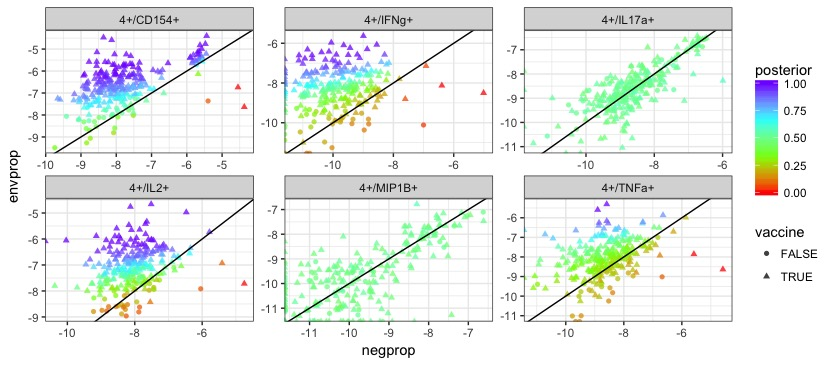
\includegraphics[width=12 cm]{figures/marginalBooleansIndependenceScatter}
 \caption{Posterior Probabilities for RV144 dataset - Independence Model}
\end{figure}
\end{center}
\end{frame}

%%%%%%%%%%%%%%%%%%%%%%%%%%%%%%%%%%%%%%%%%%%%%%%]

\begin{frame}
\frametitle{HMRF Model - Results}
\begin{figure}[]
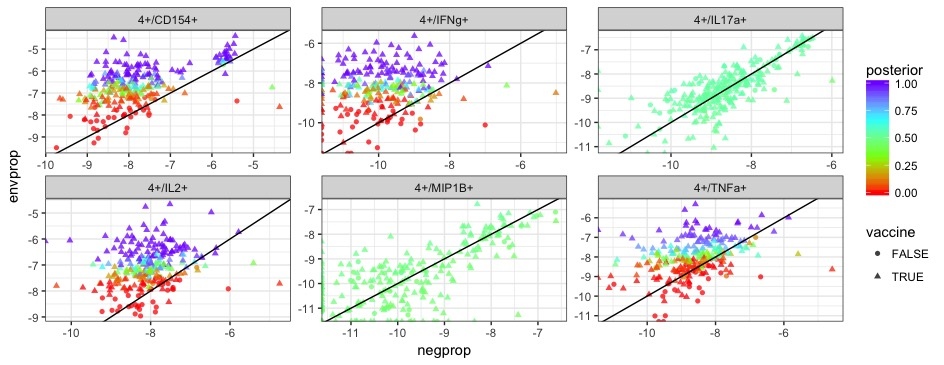
\includegraphics[width=11 cm]{figures/HMRFscatter2} \caption{Scatter Plot for HMRF Modle Model}
\end{figure}
\end{frame}

%%%%%%%%%%%%%%%%%%%%%%%%%%%%%%%%%%%%%%%%%%%%%%%]

\begin{frame}
\frametitle{Subset-Response Model - Results}
\begin{figure}[]
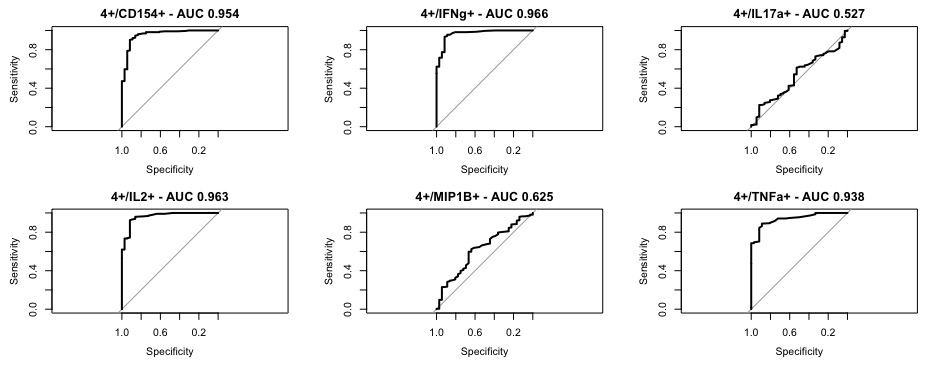
\includegraphics[width=11 cm]{figures/HMRFroc2} \caption{ROC for HMRF Modle}
\end{figure}
\end{frame}

%%%%%%%%%%%%%%%%%%%%%%%%%%%%%%%%%%%%%%%%%%%%%%%]

\begin{frame}
\frametitle{Subset-Response Model - Results}
\begin{figure}[]
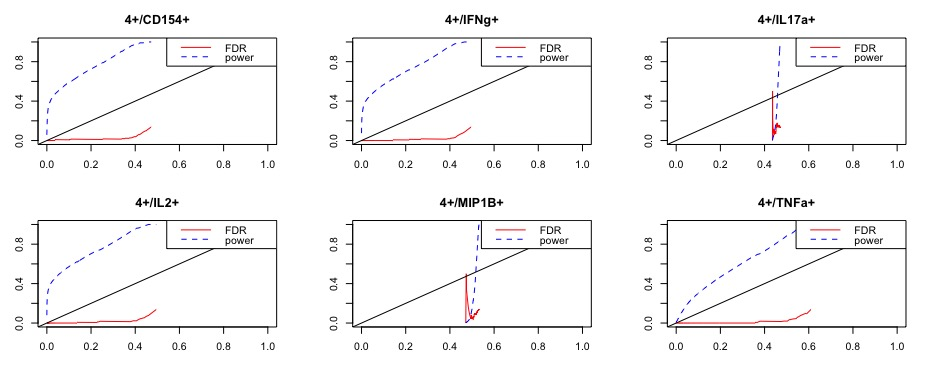
\includegraphics[width=12 cm]{figures/HMRFfdr2} \caption{FDR for HMRF Modle}
\end{figure}
\end{frame}

%%%%%%%%%%%%%%%%%%%%%%%%%%%%%%%%%%%%%%%%%%%%%%%]

\begin{frame}
\frametitle{Simulated Data Experiment}
\begin{itemize}
\item Posterior probabilities are not well calibrated.
	\begin{itemize}
	\item Might be due to true non-response.
	\end{itemize}
\pause
\vspace{0.5 cm}
\item Is the optimization algorithm estimating the model properly?
\vspace{0.5 cm}
\item Does the model fit the data well? 

\pause
\vspace{0.5 cm}
\item To find out:
	\begin{itemize}
	\item We generate data according to the estimated model.
	\item Fit should be perfect. 
	\item Is the artificial data similar to the real data?
	\end{itemize} 
\end{itemize}
\end{frame}

%%%%%%%%%%%%%%%%%%%%%%%%%%%%%%%%%%%%%%%%%%%%%%%]

\begin{frame}
\frametitle{How close are we to the distribution of the data?}
\begin{figure}[]
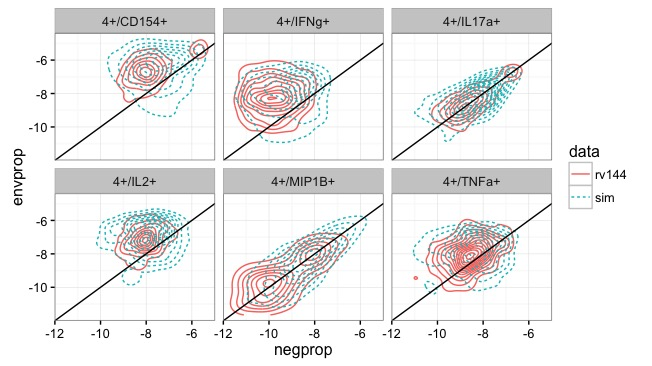
\includegraphics[width=12 cm]{figures/simVsRealContour} 
\end{figure}
\end{frame}

%%%%%%%%%%%%%%%%%%%%%%%%%%%%%%%%%%%%%%%%%%%%%%%]

\begin{frame}
\frametitle{Results for Simulated Data}
\begin{figure}[]
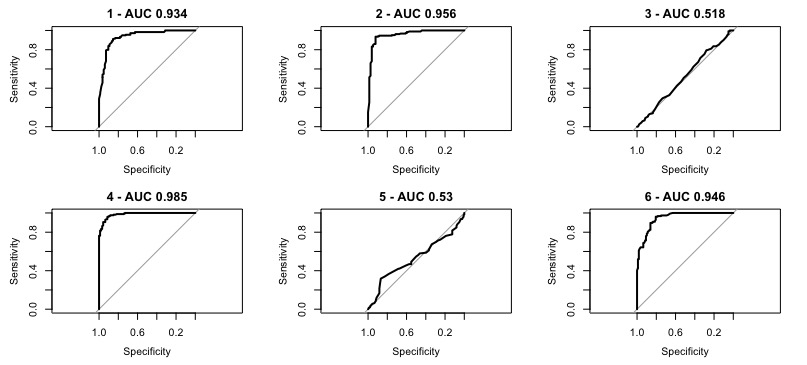
\includegraphics[width=12 cm]{figures/simdataROC} 
\end{figure}
\end{frame}

%%%%%%%%%%%%%%%%%%%%%%%%%%%%%%%%%%%%%%%%%%%%%%%]

\begin{frame}
\frametitle{Results for Simulated Data}
\begin{figure}[]
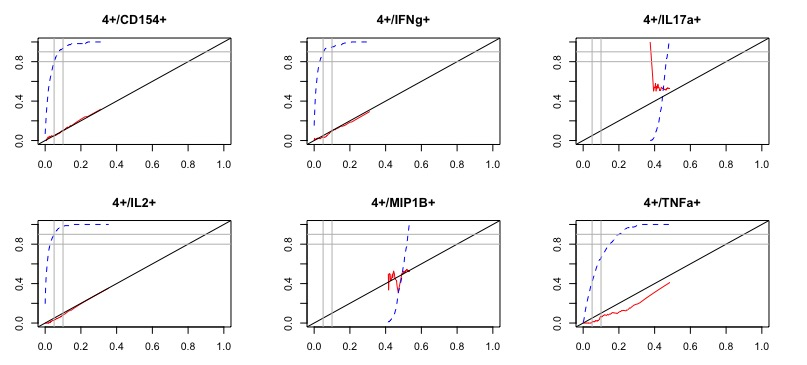
\includegraphics[width=12 cm]{figures/simdataFDR} 
\end{figure}
\end{frame}

%%%%%%%%%%%%%%%%%%%%%%%%%%%%%%%%%%%%%%%%%%%%%%%]

\begin{frame}
\frametitle{RV144 Booleans Dataset}
\begin{figure}[]
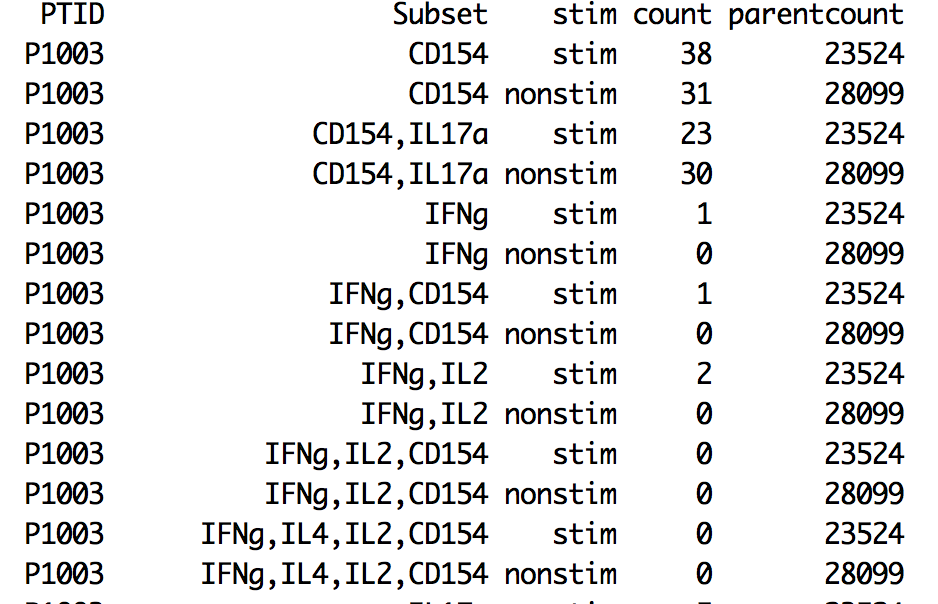
\includegraphics[width=12 cm]{figures/datasetExample} \caption{}
\end{figure}
\end{frame}

%%%%%%%%%%%%%%%%%%%%%%%%%%%%%%%%%%%%%%%%%%%%%%%]

\begin{frame}
\frametitle{RV144 Booleans Dataset}
\begin{itemize}
\item So far we worked with marginal counts - can be obtained from bulk assays. 
\pause
\vspace{0.8 cm}
\item single-cell measurements enable a more comprehensive understanding of cellular functions. 
\vspace{0.8 cm}
\item  \textbf{The degree of functionality} (numbered of expressed cytokines) of responsive cell-subsets has been correlated with favorable outcomes in vaccine studies. 
\end{itemize}
\end{frame}

%%%%%%%%%%%%%%%%%%%%%%%%%%%%%%%%%%%%%%%%%%%%%%%]

\begin{frame}
\frametitle{The RV144 Booleans Dataset}
\begin{itemize}
\item \textbf{262 Subjects}
	\begin{itemize}
	\item 226 Cases
	\item 36 Controls
	\end{itemize}
\vspace{0.2 cm}
\item \textbf{2 Types of stimulus} 
	\begin{itemize}
	\item HIV antigen
	\item Negative control
	\end{itemize}
\vspace{0.2 cm}
\item \textbf{23 types of cells with non-negligible counts.} 
	\begin{itemize}
	\item (At least two instances of \emph{count} $\geq 5$)
	\end{itemize}
\end{itemize}
\end{frame}

%%%%%%%%%%%%%%%%%%%%%%%%%%%%%%%%%%%%%%%%%%%%%%%]

\begin{frame}
\frametitle{RV144 - Booleans Dataset}
\begin{figure}[]
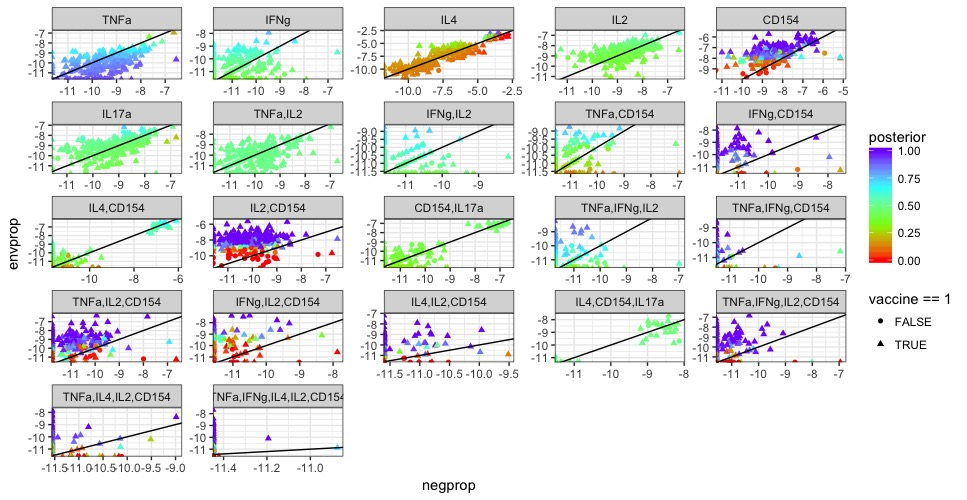
\includegraphics[width=12 cm]{figures/booleansFullScatter}
\end{figure}
\end{frame}

%%%%%%%%%%%%%%%%%%%%%%%%%%%%%%%%%%%%%%%%%%%%%%%]

\begin{frame}
\frametitle{RV144 - Booleans Dataset}
\begin{figure}[]
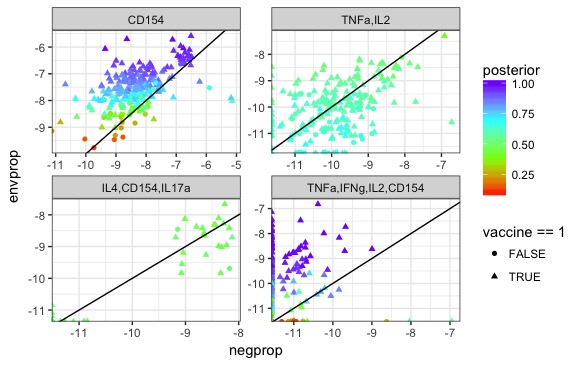
\includegraphics[width=12 cm]{figures/booleansScatterLess} 
\end{figure}
\end{frame}

%%%%%%%%%%%%%%%%%%%%%%%%%%%%%%%%%%%%%%%%%%%%%%%]

\begin{frame}
\frametitle{RV144 - Booleans Dataset}
\begin{figure}[]
\includegraphics[width=12 cm]{figures/BooleansROCless}
\end{figure}
\end{frame}

%%%%%%%%%%%%%%%%%%%%%%%%%%%%%%%%%%%%%%%%%%%%%%%]

\begin{frame}
\frametitle{RV144 - Booleans Dataset}
\begin{figure}[]
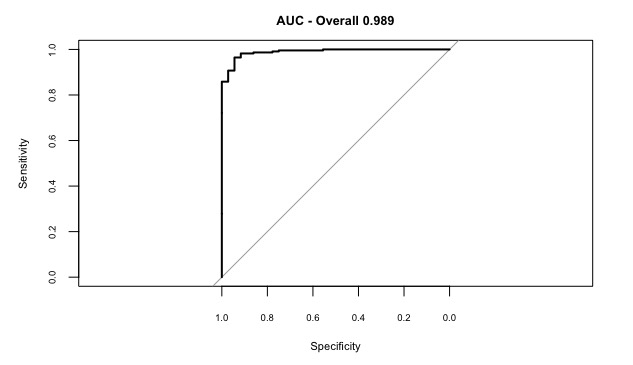
\includegraphics[width=12 cm]{figures/booleansAUCaggregate}
\end{figure}
\end{frame}

%%%%%%%%%%%%%%%%%%%%%%%%%%%%%%%%%%%%%%%%%%%%%%%]

\begin{frame}
\frametitle{RV144 - Booleans Dataset}
\begin{figure}[]
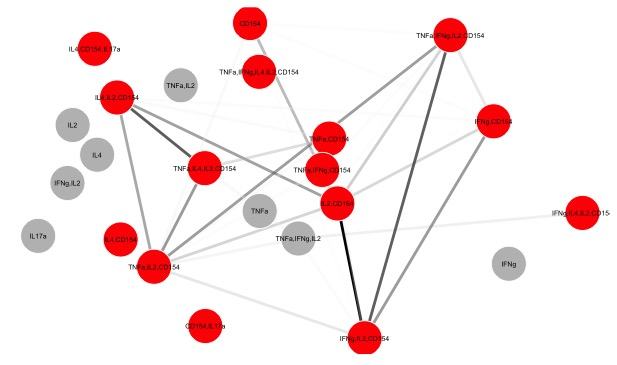
\includegraphics[width=10 cm]{figures/booleansNetworkCD154} 
\caption{Estimated Ising Model - Red marks CD154}
\end{figure}
\end{frame}

%%%%%%%%%%%%%%%%%%%%%%%%%%%%%%%%%%%%%%%%%%%%%%%]

\begin{frame}
\frametitle{RV144 - Booleans Dataset}
\begin{figure}[]
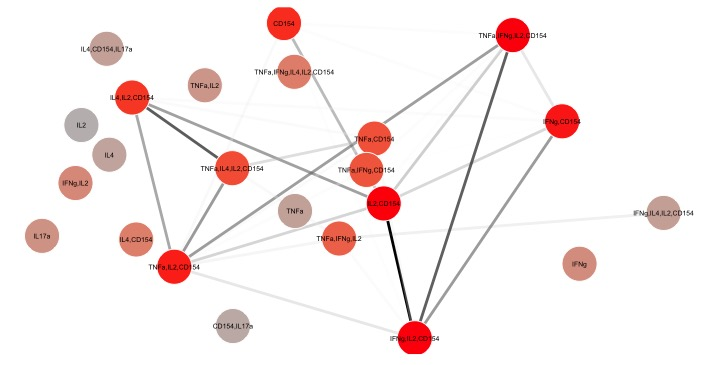
\includegraphics[width= 10.5 cm]{figures/booleansNetworkAUC} 
\caption{Estimated Ising Model - Red marks AUC}
\end{figure}
\end{frame}

%%%%%%%%%%%%%%%%%%%%%%%%%%%%%%%%%%%%%%%%%%%%%%%]


\begin{frame}
\frametitle{Controlled Human Malaria Infection Study}
\begin{figure}[]
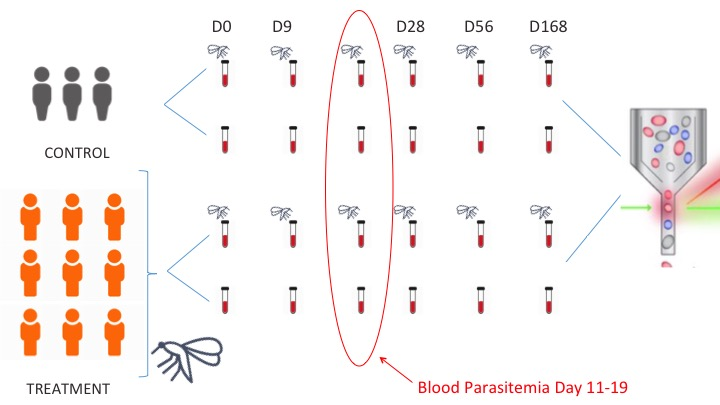
\includegraphics[width=11 cm]{figures/malariaGraphic}
\end{figure}
\end{frame}

%%%%%%%%%%%%%%%%%%%%%%%%%%%%%%%%%%%%%%%%%%%%%%%]

\begin{frame}
\frametitle{Controlled Human Malaria Infection Study}
\begin{itemize}
\item 9 subjects were infected with Malaria.
	\begin{itemize}
	\item +3 controls.
	\end{itemize}
	\vspace{0.75 cm}
	
\item Blood samples were collected at 6 time points.
	\begin{itemize}
	\item Day 0, day 9, blood  parasitemia, Day 28, Day 56, Day 168.
	\end{itemize}
	\vspace{0.75 cm}

\item Two types of stimulation:
	\begin{itemize}
	\item Infected/uninfected blood-cells.
	\end{itemize}
	\vspace{0.75 cm}
	
\item 53 cell subsets.
	\begin{itemize}
	\item (10 types of cytokines in 8 cell-types)
	\end{itemize} 
\end{itemize}
\end{frame}

%%%%%%%%%%%%%%%%%%%%%%%%%%%%%%%%%%%%%%%%%%%%%%%]

\begin{frame}
\frametitle{Controlled Human Malaria Infection Study}
\begin{itemize}
\item  Individuals  who  experience malaria  infections develop  immunity.
	\begin{itemize}
	\item All subject may exhibit response to stimulation.
	\item Even at day 0!
	\item What is the profile of the immune response?
	\end{itemize}
	
\pause
\vspace{0.5 cm}
\item The  immunity is not long lived.
	\begin{itemize}
	\item We might expect to see a rise in response during experiment.
	\item How fast does the response return to baseline?
	\end{itemize}
\end{itemize}
\end{frame}

%%%%%%%%%%%%%%%%%%%%%%%%%%%%%%%%%%%%%%%%%%%%%%%]

\begin{frame}
\frametitle{Controlled Human Malaria Infection Study}
malaraFourPlusSmoothed
\begin{figure}[]
\includegraphics[width=12 cm]{figures/fourPlusSmoothedNarrow} \caption{CD4 Helper Cells}
\end{figure}
\end{frame}

%%%%%%%%%%%%%%%%%%%%%%%%%%%%%%%%%%%%%%%%%%%%%%%]

\begin{frame}
\frametitle{FDR Adjusted p-values for CHMI Study}
Standard errors for significance tests computed using Jackknife. 
\vspace{0.4 cm}

% latex table generated in R 3.3.2 by xtable 1.8-2 package
% Thu Feb 23 03:35:46 2017
\begin{table}[ht]
\centering
\scalebox{0.65}{
\begin{tabular}{rlllllrll}
  \hline
 & 4+ & 4+/CXCR5+ & 56+dim & 56+hi & 8+ & 8+/CXCR5+ & NK T cells & PD-1+ \\ 
  \hline
154+ & \colorbox{yellow}{0.029} & \colorbox{yellow}{0.004} &  &  & 0.103 & 0.75 & \colorbox{yellow}{0.006} & \colorbox{yellow}{0.024} \\ 
  CCR7+ & 0.649 & 0.996 &  &  & 0.596 & 0.51 &  &  \\ 
  CD45A+ & 0.575 & 0.307 &  &  & 0.543 & 0.54 &  &  \\ 
  IFNg+ & \colorbox{yellow}{0.001} & \colorbox{yellow}{0.006} & \colorbox{yellow}{0.065} & 0.146 & \colorbox{yellow}{0.001} &  & \colorbox{yellow}{0.052} & \colorbox{yellow}{0.097} \\ 
  IL2+ & \colorbox{yellow}{0} & \colorbox{yellow}{0.005} &  &  & 0.119 & 0.56 & 0.321 & \colorbox{yellow}{0.052} \\ 
  IL21+ & 0.676 & 0.649 & 0.751 & 0.589 & 0.649 &  & 0.71 &  \\ 
  IL4+ & 0.12 & 0.543 &  & 0.751 & 0.649 &  & 0.583 &  \\ 
  TNFa+ & \colorbox{yellow}{0} & \colorbox{yellow}{0.001} & 0.261 & 0.309 & 0.276 &  & \colorbox{yellow}{0.053} & \colorbox{yellow}{0.09} \\ 
  GzB+ & 0.583 &  & 0.511 & \colorbox{yellow}{0.001} & 0.589 &  & 0.596 &  \\ 
  PD-1+ & 0.751 &  &  &  & 0.596 & 0.83 &  &  \\ 
   \hline
\end{tabular}}
\end{table}
\end{frame}

%%%%%%%%%%%%%%%%%%%%%%%%%%%%%%%%%%%%%%%%%%%%%%%]

\begin{frame}
\frametitle{Controlled Human Malaria Infection Study}
\begin{figure}[]
\includegraphics[width=13 cm]{figures/MalariaSignificantAt10} \caption{Significant Subsets}
\end{figure}
\end{frame}

%%%%%%%%%%%%%%%%%%%%%%%%%%%%%%%%%%%%%%%%%%%%%%%]

\begin{frame}
\frametitle{Controlled Human Malaria Infection Study}
\begin{figure}[]
\includegraphics[width=10 cm]{figures/malariaNetwork} \caption{Estimated Graph - Red marks probability of response}
\end{figure}
\end{frame}

%%%%%%%%%%%%%%%%%%%%%%%%%%%%%%%%%%%%%%%%%%%%%%%]

\begin{frame}
\frametitle{Computation - A Difficult Likelihood}
With cluster assignments and random effects known:
$$
f(y_{i} | \nu_i, k_i) = \prod_{j}\prod_{t}f(y_{ijt} | \nu_{ij}, k_{ij})
$$
\vspace{0.2 cm}

\pause
The log-likelihood of the data is given by:
$$
\ell(\beta,\tau,\theta,\Sigma) = 
\sum_{i=1}^{n}\log\left(\sum_{k\in \{0,1\}^{J}} P_\theta(k) \int_{\mathbb{R}^{J}} f_{\beta,\tau}(y_i | \nu_{i}, k_i) \varphi(\nu_i;0, \Sigma) d\nu_i\right)
$$
\vspace{0.2 cm}

The log-likelihood is intractable for large $J$. 
\end{frame}

%%%%%%%%%%%%%%%%%%%%%%%%%%%%%%%%%%%%%%%%%%%%%%%]

\begin{frame}
\frametitle{Computation - How About EM?}
The integrals are replaced with conditional expectations:
$$
\sum_{i=1}^{n}\log\left(\sum_{k\in \{0,1\}^{J}} P_\theta(k | y_i) \int_{\mathbb{R}^{J}} f_{\beta,\tau}(y_i | \nu_{i}, k_i) f_{\Sigma}(\nu_i| y_i, k) d\nu_i\right)
$$

\pause
\vspace{0.3 cm}
We can use sampling to approximate the intractable integrals:
$$
k_{i1}^*,...,k_{iM}^* \sim P_\theta(k|y_i)
$$$$
\nu_{i1}^* \sim f(\nu_i|y_i, k_{i1}),...,\nu_{iM}^* \sim f(\nu_i|y_i, k_{iM})
$$$$
(\beta, \tau, \theta, \Sigma) = \arg\max \sum_{i=1}^{n}\frac{1}{M}\sum_{m=1}^{M} \sum_{j} \sum_{t} \log f(y_{ijt} | \nu_{im}^{*}, k_{im}^{*})
$$
\end{frame}

%%%%%%%%%%%%%%%%%%%%%%%%%%%%%%%%%%%%%%%%%%%%%%%]

\begin{frame}
\frametitle{Computation - Stochastic EM Algorithm}
We alternate between a stochastic E-step and an M-step. 



\vspace{0.75 cm}
\textbf{S - Step}
\begin{itemize}
\item $\boldsymbol{k^*}$ - Gibbs sampler.
\item $\boldsymbol{\nu^* | k^*}$ - component-wise MH algorithm. 
\end{itemize}


\vspace{0.75 cm}
\textbf{M - Step}
\begin{itemize}
\item $\boldsymbol{\beta, \tau}$ - \textbf{glm, glmnet} for sparsity or \textbf{gamlss} for BB.
\item $\boldsymbol{\theta}$ - Pseudo-likelihood or \textbf{isingFit} for sparsity .
\item $\boldsymbol{\Sigma}$ - Option for sparse estimation via \textbf{PSDE} package.
\end{itemize}
\end{frame}

%%%%%%%%%%%%%%%%%%%%%%%%%%%%%%%%%%%%%%%%%%%%%%%]

\begin{frame}
\begin{center}
\huge{Thank you!}

\vspace{2 cm}
\LARGE{Questions?}

\vspace{1cm}
\large{AmitMeir@uw.edu}
\end{center}
\end{frame}


\end{document}
